\section{Discussion}
This section focuses on discussing the previously presented results in Experiment 2.

\subsection{Relationships Between Alignment Fail Rates and Mean Number of Resets}\label{sec:orbitalCases}
\begin{figure}[tbph]
    \centering
    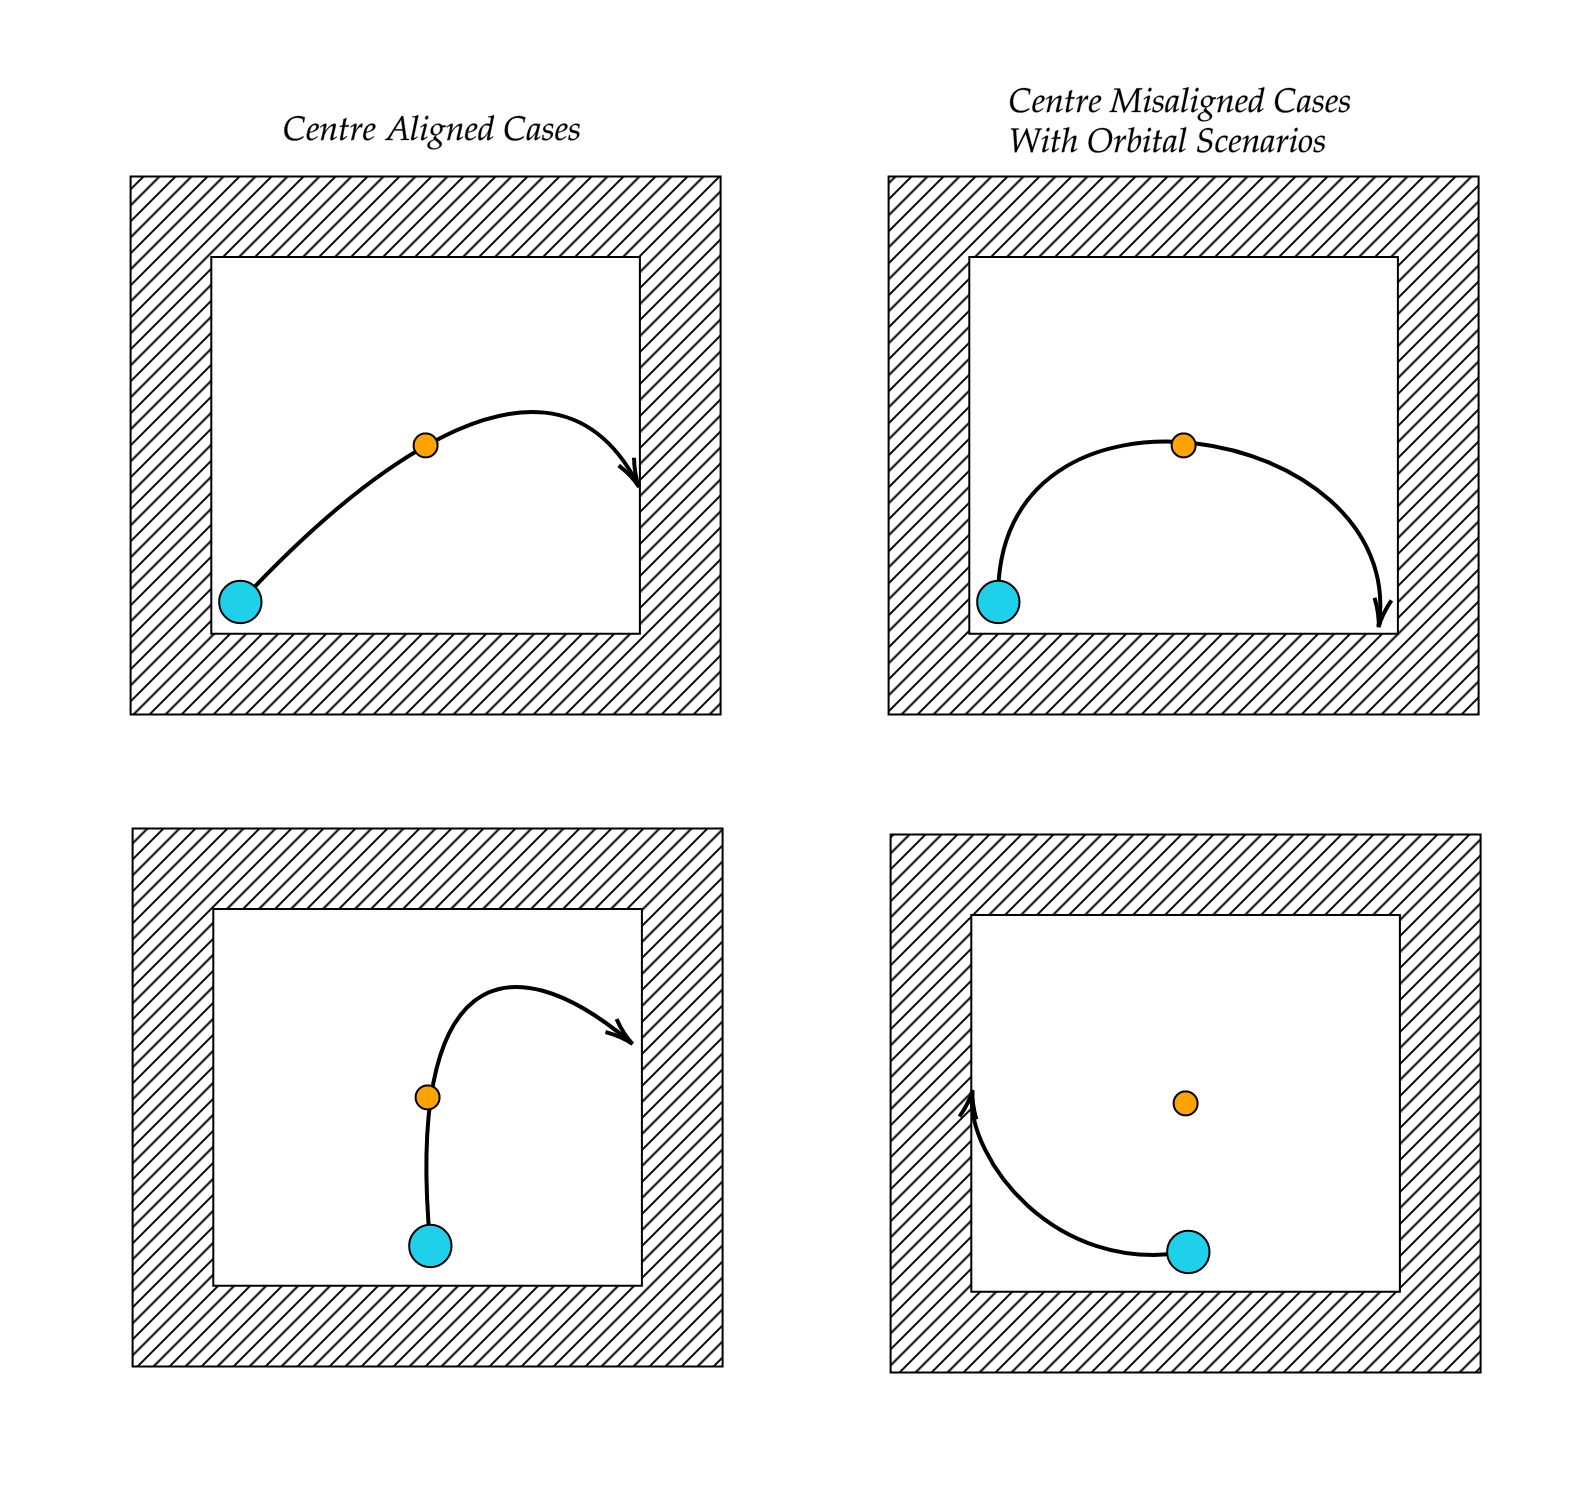
\includegraphics[width=0.9\textwidth]{figures/graphs/orbitalcases.png}
    \caption[Illustration of Various S2C Redirection Scenarios During Success/Failure of Centre Alignment]{This illustration shows some expected paths that the user can take when using the S2C Algorithm after finishing distractor interaction. For the sake of these illustrations, only curvature gain is considered as the user is not expected to move their head much when walking towards a goal. The illustration also focuses on virtual straight walking situations specifically. Failure to align the user to centre during distraction can result in ''orbital scenarios''. The effectiveness of these will vary depending on where in the room the user is before starting to walk again.}
    \label{fig:orbitalCases}
\end{figure}

One of the most interesting results from Experiment 2 is that there was no significant difference in terms of mean number of resets, but there was a $15.8\%$ difference in fail rates. Given the higher fail rate for using S2C only, it would be expected that this condition in general results in more resets as it fails to align the user to the centre. The question then becomes: why is this not the case? It may be that while only using S2C results in more failures to fully align the user towards the centre, it may be close enough to avoid them moving into the reset bounds of nearby walls. Of course, the results may also just be like they are due to the sample size, but thinking about the current results provides some interesting ideas. 

\subsubsection{''Orbital Scenarios''}
While this is just speculation, if the user is at the corner of a room and starts to walk parallel to a wall rather than towards the centre, it may result in longer curved paths. This is illustrated in Figure~\ref{fig:orbitalCases} in what we could consider an ''orbital scenario''. The illustration relies on curvature gains only as the amount of head rotation while walking is generally limited. To show an example of the differences in head rotation between walking and battle states, see Figure~\ref{fig:ex2headRotationAuthor} and the supplementary Figure~\ref{fig:ex2DeltaTimeAuthor}. The first of these shows the changes in head rotation throughout the experiment while the author participated and the second figure shows the related frame latencies between the two states. The frame latencies between the two states appear to be relatively similar and as such, should not have an impact on Figure~\ref{fig:ex2headRotationAuthor}.

The effectiveness of the aforementioned orbital scenarios would likely vary depending on where in the room the user is after distraction is finished. One of these cases consists of the user starting in a corner space and starting to walk roughly in parallel with any walls. When this happens, they will likely go a further distance until the next distractor triggers compared to if they walked straight towards the centre. The reasoning for this is that S2C as an algorithm will not attempt to apply any curvature gains while moving towards the room centre. As such the amount of effective redirection is roughly halved as redirection is not applied until the user has moved past the centre again. On the other hand, if the user starts at the middle point of a wall and moves roughly in parallel with it, they will likely hit a distractor or reset trigger quite a bit earlier compared to if they started to move towards the centre of the room.  

Due to this potentially happening, it could explain why the fail rate is different while the mean number of resets between conditions is not. If using S2C only results in optimal orbital scenarios at times, while being slightly more inefficient otherwise, the total effectiveness for using S2C only could average out and become similar to S2C+AC2F.

\subsubsection{Optimising the S2C Algorithm During Straight Walking When Using S2C+AC2F}
Given the possibility of orbital scenarios, the overall solution of using distractors could be somewhat optimised. It should be noted that this optimisation would work assuming S2C is employed during walking and AC2F is used with distractors. In cases where users will walk in straight lines, we could dynamically create the alignment heuristic depending on where they are physically located instead of always aligning to centre. By optimising the alignment heuristic that AC2F aims to align towards, S2C can provide a more effective curved path after distractor interaction is finished. To some extent, this would result in similar movement to the Steer To Orbit(S2O) algorithm whenever this is optimal. Given that S2O primarily outperforms S2C for physical spaces between $16m^2$ and $31m^2$~\cite{azmandian2015physical}, the focus should ideally lie on optimising the walking paths of S2C. This is largely due to current day physical spaces being small enough that S2C is more efficient than S2O.   

Furthermore, it is important to keep in mind that this optimisation would primarily apply to straight walking scenarios when using S2C+AC2F. If straight walking is not expected in the developed experience, it may both be safer and more efficient to simply always set the AC2F heuristic to align to centre. Regardless, it is an interesting thought to entertain in terms of how S2C+AC2F can be improved as a whole. 

\subsubsection{Mitigating Failure Cases for the AC2F Algorithm}
Another element that can be further optimised is to mitigate the failure cases for the AC2F algorithm. The results show that AC2F only fails during the shortest distractor battles as the player's baton at those points is at the highest damage level. Furthermore, the main reasoning behind these failures is insufficient head rotation which can only happen if the distractor chooses small random angles to move in. AC2F as an algorithm will always succeed alignment given enough head rotation for any specific situation. S2C on the other hand will not necessarily do this if used in place of AC2F as it does not consider the alignment heuristic that AC2F does. It could be possible to mitigate AC2F's failure cases by introducing a minimum angle for distractor movement rather than using pure randomness. By doing so, we can guarantee that a certain amount of head movement will happen and as such, make sure that the failure rate decreases for the shortest battles. This is of course a rather specific optimisation to the usage of one type of concrete distractors. Despite this, it would be a great benefit whenever a virtual experience makes use of concrete distractors that rely on movement to facilitate head rotation. 

\subsection{Potential Improvements to the Data Processing Approach}
Another side of Experiment 2 that could be substantially improved is to streamline and improve the data processing approach. Currently, there is a large amount of post processing needed to get relevant and usable data which technically could have been recorded more easily and automatically on the software side of Ensemble Retriever. Furthermore, the processing of unintentional resets could also be improved. Instead of cutting off all resets that happen within the first 10 seconds of a distractor spawn, it might be more accurate to instead only \emph{include} resets that happen within the last 10 seconds of a distractor's life. This would likely be a better approach to removing type 2 unintentional resets which were mentioned in Section~\ref{sec:ex2postprocessing}. In the current approach it is possible to for example have a distractor last for 50 seconds and have an type 2 unintentional reset at 25 seconds due to large amounts of engaged movement. With the current approach, this reset would have been recorded as legitimate instead of unintentional. Fixing this in post processing would be rather challenging due to the time serial data format, but doing so on the software side of the recording should be rather feasible. 

The need to perform this post processing in the first place came from observing human factors and behaviour that were attempted to be mitigated from Experiment 1. In particular, mitigating type 1 unintentional resets was the main reasoning behind increasing the buffer between reset and distractor trigger bounds. While this change in general likely mitigated a good amount of unintentional resets, it did not fully stop them from happening. It would of course be possible to further increase the buffer, but this would risk having the actual walkable space become smaller and more annoying for participants as distractors would trigger with higher frequency. Providing more accuracy in terms of being able to remove unintentional resets would likely help with providing more valid and accurate results. 

\subsection{Minimising the Risk of Cybersickness Buildup With Distractors}\label{sec:ex2MinimisingCybersickness}

The results from Experiment 2 showed that the mean time needed for alignment in successful cases for AC2F was \textasciitilde23 seconds. At the same time, the mean time needed to defeat a distractor at the highest baton level was \textasciitilde42 seconds. This provides an interesting time buffer which could be used in a variety of ways. One possibility would be to decrease the employed rotation gains so they better fit the length of a distractors life. This would likely contribute to decreasing the risk of hitting various individuals' cybersickness thresholds. Another option would be to keep the current gains and instead decrease the time needed to interact with distractors. 

Decreasing the strength of rotation gains would result in longer periods of exposure to redirection. In comparison, if the gains are strong, then alignment will happen earlier and disable redirection until the distractor is finished. Which of these two approaches is ideal in terms of cybersickness is hard to say, but it would have been interesting to see future research look into it. Another element that these two approaches could affect is the adaptation towards positive rotation gains which were experienced in Experiment 1. If there are little to no periods of time where 0 gains are applied to the user, then this might result in different adaptation effects compared to what was experienced in Experiment 1. This is also something that would be interesting to see further research on.

One thing that should be noted though is that lowering the gains will likely have a negative effect on the alignment failures that are experienced in shorter battles. If the improvements discussed in Section~\ref{sec:orbitalCases} were to be implemented, then this would likely make it easier to decrease gains without impacting alignment failure rates to the same degree. In general though, it would be recommended to still have some buffer between the time needed to defeat distractors and the time needed for alignment in case of unforeseen circumstances.
   
From a game design point of view, the results show that the majority of the gameplay time is spent on battles. In cases where more exploration is necessary, it might be better for the players to actually spend less time fighting distractors and more time on walking around. From this perspective, stronger gains with shorter battles would be ideal. 
   
\subsection{Success of Employing Mean Detection Threshold Gains From Experiment 1}
The employed redirection gains in Experiment 2 were derived from mean detection thresholds in Experiment 1. Despite these thresholds being aggregates from rather diverse individuals, the results seem to point towards this approach having been relatively successful. In terms of qualitative feedback, 6 out of 13 mentioned they had noticed they were being redirected at some points during the experience. Despite this, no participants mentioned feeling any cybersickness or nausea as a result from the redirection. As such, it would not appear that the cybersickness thresholds for the individual participants in the sample were exceeded. Employing the same gains for a different population might not have worked quite as well though, as the mean detection thresholds could vary and so could the cybersickness thresholds. The approach of using detection thresholds for redirection gains to strike a balance between effectiveness and comfort will likely only be safe if the gains are derived from estimated thresholds of the target population. Furthermore, since there were no direct cybersickness tests in this experiment, it is hard to fully conclude the effectiveness of the approach other than that uncomfortable levels were not reached.  

\subsection{Correlation Matrix Discussion}\label{sec:ex2correlationAnalysis}
This section will further analyse the significant correlations that were found in Figure~\ref{fig:ex2correlation1} and~\ref{fig:ex2correlation2}. 

\subsubsection{Correlations for Age Range}
There are a few significant negative correlations for the age range variable. There is little information that can be gained from these as the vast majority of the participant sample was within the age range of 18-24. 

\subsubsection{Correlations for Prior VR Experience}
In terms of prior VR experience, there appears to be a negative correlation in terms of time spent walking. There is little additional analysis that can be done on this. 

One area where this variable has a positive correlation though is on the mean walking speed of participants. If we take a look at Figure~\ref{fig:meanWalkingSpeedAndPriorExperience}, there appears to be a general trend on walking speeds increasing as higher amounts of prior VR experience is reported. The distribution for this sample is rather skewed towards those reporting a value of 1 and 5 though so drawing any major conclusions on this hard. It would not necessarily be surprising that higher amounts of experience relates to participants that are comfortable with higher movement speeds in VR though.

\subsubsection{Correlations for Time Spent Walking}
One interesting negative correlation is between time spent walking and the mean movement speed. In general, it would be expected that higher walking speeds would correlate to less time spent on walking. Despite this, there is a limitation with the recording of the time spent walking variable that likely results in this negative correlation. Time spent walking as a variable is calculated by looking at the time that was not spent in distractor battles. As such, it can also consist of time spent on simply standing still and looking around outside of battles. 

\subsubsection{Correlations for Number of Legitimate Resets}
The number of legitimate resets is negatively correlated with the number of failed alignments. This is not particularly surprising as the two variables are not really related to each other. The number of failed alignments as a variable primarily relates to the level of the participants' baton as well as the amount of random movement that a distractor does. 

\subsubsection{Correlations for Time Taken Until Alignment}
For the time taken until alignment, there is a negative correlation in terms of age range, but as already mentioned there is little information to gain from this.


